%%%%%%%%%%%%%%%%%%%%%%%%%%%%%%%%%%%%%%%%%%%%%%%%%%%%%%%%%%%%%%%%%%%%%%%%%%%%%%
%% Copyright 2014 Thiago Nascimento											%%
%% 																			%%
%% Licensed under the Apache License, Version 2.0 (the "License");			%%
%% you may not use this file except in compliance with the License.			%%
%% You may obtain a copy of the License at									%%
%% 																			%%
%%     http://www.apache.org/licenses/LICENSE-2.0							%%
%%     																		%%
%% Unless required by applicable law or agreed to in writing, software		%%
%% distributed under the License is distributed on an "AS IS" BASIS,		%%
%% WITHOUT WARRANTIES OR CONDITIONS OF ANY KIND, either express or implied.	%%
%% See the License for the specific language governing permissions and		%%
%% limitations under the License.											%%
%%																			%%
%%%%%%%%%%%%%%%%%%%%%%%%%%%%%%%%%%%%%%%%%%%%%%%%%%%%%%%%%%%%%%%%%%%%%%%%%%%%%%

%%%%%%%%%%%%%%%%%%%%%%%%%%%%%%%%%%%%%%%%%%%%%%%%%%%%%%%%%%%%%%%%%%%%%%%%%%%%%%
%% Modelo de trabalho acadêmico para Mestrado Acadêmico e Profissional		%%
%% da Universidade Estadual do Ceará - UECE									%%
%%																			%%
%% Autor: Thiago Nascimento													%%
%%																			%%
%% Projeto hospedado em: https://github.com/thiagodnf/abntex2-uece			%%
%%																			%%
%% Informações:																%%
%%		Codificação utilizada: UTF-8										%%
%%  	Tamanho da tabulação: 4 (espaços)									%%
%%%%%%%%%%%%%%%%%%%%%%%%%%%%%%%%%%%%%%%%%%%%%%%%%%%%%%%%%%%%%%%%%%%%%%%%%%%%%%

% % % % % % % % % % % % % % % % % % % % % % % % % % % % % % % % % % % % % % % 
%																			%
% 		Obs.: Deixe o campo em branco quando não existir a informação 		%
%																			%
% % % % % % % % % % % % % % % % % % % % % % % % % % % % % % % % % % % % % % %

\documentclass[a4paper,12pt,oneside]{abntex2}

% Importações de pacotes
\usepackage[alf, abnt-emphasize=bf, bibjustif, recuo=0cm, abnt-etal-cite=2, abnt-etal-list=0]{abntex2cite}  % Citações padrão ABNT
\usepackage[utf8]{inputenc}                         % Acentuação direta
\usepackage[T1]{fontenc}                            % Codificação da fonte em 8 bits
\usepackage{graphicx}                               % Inserir figuras
\usepackage{amsfonts, amssymb, amsmath}             % Fonte e símbolos matemáticos
\usepackage{booktabs}                               % Comandos para tabelas
\usepackage{verbatim}                               % Texto é interpretado como escrito no documento
\usepackage{multirow, array}                        % Múltiplas linhas e colunas em tabelas
\usepackage{indentfirst}                            % Endenta o primeiro parágrafo de cada seção.
\usepackage{microtype}                              % Para melhorias de justificação?
\usepackage[algoruled, portuguese]{algorithm2e}     % Escrever algoritmos
\usepackage{float}                                  % Utilizado para criação de floats
\usepackage{amsgen}
%\usepackage[bottom]{footmisc}                      % Mantém as notas de rodapé sempre na mesma posição
%\usepackage{times}                                 % Usa a fonte Times
\usepackage{mathptmx}                               % Usa a fonte Times New Roman										
%\usepackage{lmodern}                               % Usa a fonte Latin Modern
%\usepackage{subfig}                                % Posicionamento de figuras
%\usepackage{scalefnt}                              % Permite redimensionar tamanho da fonte
%\usepackage{color, colortbl}                       % Comandos de cores
%\usepackage{lscape}                                % Permite páginas em modo "paisagem"
%\usepackage{ae, aecompl}                           % Fontes de alta qualidade
%\usepackage{picinpar}                              % Dispor imagens em parágrafos
%\usepackage{latexsym}                              % Símbolos matemáticos
%\usepackage{upgreek}                               % Fonte letras gregas
\usepackage{modelo/abtnex2-uece-dissertacao}		% Biblioteca com as normas da UECE para dissertações

%%%%%%%%%%%%%%%%%%%%%%%%%%%%%%%%%%%%%%%%%%%%%%%%%%%%%
%% 			 Informação sobre o Curso			   %%
%%%%%%%%%%%%%%%%%%%%%%%%%%%%%%%%%%%%%%%%%%%%%%%%%%%%%

\ies{Universidade Estadual do Ceará}
\centro{Centro de Ciência e Tecnologia}
\programa{Programa de Pós-Graduação em Ciência da Computação}
\mestrado{Mestrado Acadêmico em Ciência da Computação}
\curso{Curso de Ciência da Computação}
\mestreem{Ciência da Computação}

% Se o seu mestrado tem area de concentracao
% Exemplo: \areadeconcetracao{Área de Concentração: Saúde Coletiva.} 
\areadeconcetracao{}

%%%%%%%%%%%%%%%%%%%%%%%%%%%%%%%%%%%%%%%%%%%%%%
%% 	Informação relacionadas a dissertação   %%
%%%%%%%%%%%%%%%%%%%%%%%%%%%%%%%%%%%%%%%%%%%%%%

\autor{Nome Sobrenome}
\titulo{Título do Trabalho}
\data{2014}
\local{Fortaleza -- Ceará}

% Exemplo: \dataaprovacao{01 de Janeiro de 2012}
\dataaprovacao{}

%%%%%%%%%%%%%%%%%%%%%%%%%%%%%%%%%%%%%%%%%%%%%
%% 		Informação sobre o Orientador	   %%
%%%%%%%%%%%%%%%%%%%%%%%%%%%%%%%%%%%%%%%%%%%%%

\orientador{Nome do seu Orientador}
\orientadories{Universidade Estadual do Ceará – UECE}

%%%%%%%%%%%%%%%%%%%%%%%%%%%%%%%%%%%%%%%%%%%%%
%% 		Informação sobre o Co-orientador   %%
%%%%%%%%%%%%%%%%%%%%%%%%%%%%%%%%%%%%%%%%%%%%%

\coorientador{}
\coorientadories{}

%%%%%%%%%%%%%%%%%%%%%%%%%%%%%%%%%%%%%%%%%%%%%
%% 		Informação sobre a banca		   %%
%%%%%%%%%%%%%%%%%%%%%%%%%%%%%%%%%%%%%%%%%%%%%

% Atenção! Se o seu trabalho tem coorientador, as informações sobre o
% membro da banca Dois serão desconsideradas.

% Exemplo:
% \membrodabancadois{Prof. Dr. Fulano de Tal}
% \membrodabancadoisies{Universidade Estadual do Ceará - UECE}

\membrodabancadois{Membro da Banca Dois}
\membrodabancadoisies{Universidade do Membro da Banca Dois}
\membrodabancatres{Membro da Banca Três}
\membrodabancatresies{Universidade do Membro da Banca Três}
\membrodabancaquatro{}
\membrodabancaquatroies{}

\dedicatoriaa{
	Dedico este trabalho a...	
}

\begin{document}
	% Retira espaço extra obsoleto entre as frases.
	\frenchspacing
	
	% Elementos pré-textuais
	\imprimircapa
	\imprimirfolhaderosto{}
	\imprimirfolhadeaprovacao
	\imprimirdedicatoria
	
	%Elementos textuais
	\chapter{Introdução}
\label{chap:introducao}

\lipsum[2]

\begin{figure}[h!]
	\caption{Mapa conceitual do estudo da história e relações com o objeto de estudo}
	\label{fig_mapa}
	\begin{center}
		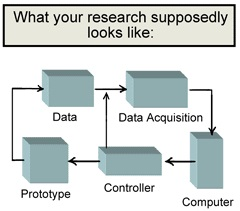
\includegraphics[width=8cm]{capitulos/figuras/figura-1}		
	\end{center}
	\fontedafigura{8cm}{os autores}
\end{figure}

\lipsum[2]
\lipsum[2]
\lipsum[2]

\begin{figure}[h!]
	\caption{Paradigma segundo processos que caracterizam a EFSFVS como Escola do SUS}
	\label{fig_paradigma}
	\begin{center}
		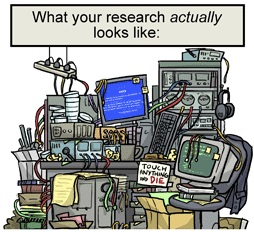
\includegraphics[width=8cm]{capitulos/figuras/figura-2}
	\end{center}
	\fontedafigura{8cm}{Adaptado de}
\end{figure}

\lipsum[2]
\lipsum[2]

\section{Motivação}
\lipsum[2]
\lipsum[2]

\section{Objetivos}

\lipsum[2]
\lipsum[2]
\lipsum[2]
\lipsum[2]
\lipsum[2]
\begin{table}[h!]	
	\caption{Internal exon scores}
	\label{tab:internal}
	\centering
	\begin{tabular}{|c|l|l|}
		\hline
		Ranking & Exon Coverage & Splice Site Support\\
		\hline
		E1 & Complete coverage by a single transcript & Both splice sites\\
		E2 & Complete coverage by more than a single transcript & Both splice sites\\
		E3 & Partial coverage & Both splice sites\\
		E4 & Partial coverage & One splice site\\
		E5 & Complete or partial coverage & No splice sites\\
		E6 & No coverage & No splice sites\\
		\hline
	\end{tabular}
	\fontedatabela{14.6cm}{os autores}
\end{table}

\lipsum[2]
\subsection{Objetivo Geral}
\lipsum[2]

\subsection{Objetivos Específicos}
	\lipsum[2]
	
	\begin{alineas}
		\item \lipsum[2]
		\item \lipsum[2]
		\begin{alineas}
			\item \lipsum[2]
			\item \lipsum[2]
		\end{alineas}
		\item \lipsum[2]	
	\end{alineas}
	
	\lipsum[2]
\subsubsection{Objetivo Geral}
	\lipsum[2]
	
\subsubsection{Objetivo Geral}
	\lipsum[2]
	\acrlong{DATASUS},\acrlong{DNV},\acrlong{DO},\acrlong{ESF},\acrlong{IBGE},\acrlong{MFC},\acrlong{MI},\acrlong{MS},\acrlong{NV},\acrlong{ODM},\acrlong{OI},\acrlong{OMS},\acrlong{ONU},\acrlong{PNI},\acrlong{PSF},\acrlong{RIPSA},\acrlong{RN},\acrlong{SIM},\acrlong{SINASC},\acrlong{SUS},\acrlong{TMI},\acrlong{TMMFC}
	
	
	%Elementos pós-textuais	

\end{document}